\documentclass[11pt,a4paper,]{article}
\usepackage{lmodern}

\usepackage{amssymb,amsmath}
\usepackage{ifxetex,ifluatex}
\usepackage{fixltx2e} % provides \textsubscript
\ifnum 0\ifxetex 1\fi\ifluatex 1\fi=0 % if pdftex
  \usepackage[T1]{fontenc}
  \usepackage[utf8]{inputenc}
\else % if luatex or xelatex
  \usepackage{unicode-math}
  \defaultfontfeatures{Ligatures=TeX,Scale=MatchLowercase}
\fi
% use upquote if available, for straight quotes in verbatim environments
\IfFileExists{upquote.sty}{\usepackage{upquote}}{}
% use microtype if available
\IfFileExists{microtype.sty}{%
\usepackage[]{microtype}
\UseMicrotypeSet[protrusion]{basicmath} % disable protrusion for tt fonts
}{}
\PassOptionsToPackage{hyphens}{url} % url is loaded by hyperref
\usepackage[unicode=true]{hyperref}
\hypersetup{
            pdftitle={ETC5513-Assignment4},
            pdfborder={0 0 0},
            breaklinks=true}
\urlstyle{same}  % don't use monospace font for urls
\usepackage{geometry}
\geometry{a4paper, centering, text={16cm,24cm}}
\usepackage[style=authoryear-comp,]{biblatex}
\addbibresource{references.bib}
\usepackage{longtable,booktabs}
% Fix footnotes in tables (requires footnote package)
\IfFileExists{footnote.sty}{\usepackage{footnote}\makesavenoteenv{long table}}{}
\usepackage{graphicx,grffile}
\makeatletter
\def\maxwidth{\ifdim\Gin@nat@width>\linewidth\linewidth\else\Gin@nat@width\fi}
\def\maxheight{\ifdim\Gin@nat@height>\textheight\textheight\else\Gin@nat@height\fi}
\makeatother
% Scale images if necessary, so that they will not overflow the page
% margins by default, and it is still possible to overwrite the defaults
% using explicit options in \includegraphics[width, height, ...]{}
\setkeys{Gin}{width=\maxwidth,height=\maxheight,keepaspectratio}
\IfFileExists{parskip.sty}{%
\usepackage{parskip}
}{% else
\setlength{\parindent}{0pt}
\setlength{\parskip}{6pt plus 2pt minus 1pt}
}
\setlength{\emergencystretch}{3em}  % prevent overfull lines
\providecommand{\tightlist}{%
  \setlength{\itemsep}{0pt}\setlength{\parskip}{0pt}}
\setcounter{secnumdepth}{5}

% set default figure placement to htbp
\makeatletter
\def\fps@figure{htbp}
\makeatother


\title{ETC5513-Assignment4}

%% MONASH STUFF

%% CAPTIONS
\RequirePackage{caption}
\DeclareCaptionStyle{italic}[justification=centering]
 {labelfont={bf},textfont={it},labelsep=colon}
\captionsetup[figure]{style=italic,format=hang,singlelinecheck=true}
\captionsetup[table]{style=italic,format=hang,singlelinecheck=true}


%% FONT
\RequirePackage{bera}
\RequirePackage[charter,expert,sfscaled]{mathdesign}
\RequirePackage{fontawesome}

%% HEADERS AND FOOTERS
\RequirePackage{fancyhdr}
\pagestyle{fancy}
\rfoot{\Large\sffamily\raisebox{-0.1cm}{\textbf{\thepage}}}
\makeatletter
\lhead{\textsf{\expandafter{\@title}}}
\makeatother
\rhead{}
\cfoot{}
\setlength{\headheight}{15pt}
\renewcommand{\headrulewidth}{0.4pt}
\renewcommand{\footrulewidth}{0.4pt}
\fancypagestyle{plain}{%
\fancyhf{} % clear all header and footer fields
\fancyfoot[C]{\sffamily\thepage} % except the center
\renewcommand{\headrulewidth}{0pt}
\renewcommand{\footrulewidth}{0pt}}

%% MATHS
\RequirePackage{bm,amsmath}
\allowdisplaybreaks

%% GRAPHICS
\RequirePackage{graphicx}
\setcounter{topnumber}{2}
\setcounter{bottomnumber}{2}
\setcounter{totalnumber}{4}
\renewcommand{\topfraction}{0.85}
\renewcommand{\bottomfraction}{0.85}
\renewcommand{\textfraction}{0.15}
\renewcommand{\floatpagefraction}{0.8}


%\RequirePackage[section]{placeins}

%% SECTION TITLES


%% SECTION TITLES
\RequirePackage[compact,sf,bf]{titlesec}
\titleformat*{\section}{\Large\sf\bfseries\color[rgb]{0.7,0,0}}
\titleformat*{\subsection}{\large\sf\bfseries\color[rgb]{0.7,0,0}}
\titleformat*{\subsubsection}{\sf\bfseries\color[rgb]{0.7,0,0}}
\titlespacing{\section}{0pt}{2ex}{.5ex}
\titlespacing{\subsection}{0pt}{1.5ex}{0ex}
\titlespacing{\subsubsection}{0pt}{.5ex}{0ex}


%% TITLE PAGE
\def\Date{\number\day}
\def\Month{\ifcase\month\or
 January\or February\or March\or April\or May\or June\or
 July\or August\or September\or October\or November\or December\fi}
\def\Year{\number\year}

%% LINE AND PAGE BREAKING
\sloppy
\clubpenalty = 10000
\widowpenalty = 10000
\brokenpenalty = 10000
\RequirePackage{microtype}

%% PARAGRAPH BREAKS
\setlength{\parskip}{1.4ex}
\setlength{\parindent}{0em}

%% HYPERLINKS
\RequirePackage{xcolor} % Needed for links
\definecolor{darkblue}{rgb}{0,0,.6}
\RequirePackage{url}

\makeatletter
\@ifpackageloaded{hyperref}{}{\RequirePackage{hyperref}}
\makeatother
\hypersetup{
     citecolor=0 0 0,
     breaklinks=true,
     bookmarksopen=true,
     bookmarksnumbered=true,
     linkcolor=darkblue,
     urlcolor=blue,
     citecolor=darkblue,
     colorlinks=true}

\usepackage[showonlyrefs]{mathtools}
\usepackage[no-weekday]{eukdate}

%% BIBLIOGRAPHY

\makeatletter
\@ifpackageloaded{biblatex}{}{\usepackage[style=authoryear-comp, backend=biber, natbib=true]{biblatex}}
\makeatother
\ExecuteBibliographyOptions{bibencoding=utf8,minnames=1,maxnames=3, maxbibnames=99,dashed=false,terseinits=true,giveninits=true,uniquename=false,uniquelist=false,doi=false, isbn=false,url=true,sortcites=false}

\DeclareFieldFormat{url}{\texttt{\url{#1}}}
\DeclareFieldFormat[article]{pages}{#1}
\DeclareFieldFormat[inproceedings]{pages}{\lowercase{pp.}#1}
\DeclareFieldFormat[incollection]{pages}{\lowercase{pp.}#1}
\DeclareFieldFormat[article]{volume}{\mkbibbold{#1}}
\DeclareFieldFormat[article]{number}{\mkbibparens{#1}}
\DeclareFieldFormat[article]{title}{\MakeCapital{#1}}
\DeclareFieldFormat[article]{url}{}
%\DeclareFieldFormat[book]{url}{}
%\DeclareFieldFormat[inbook]{url}{}
%\DeclareFieldFormat[incollection]{url}{}
%\DeclareFieldFormat[inproceedings]{url}{}
\DeclareFieldFormat[inproceedings]{title}{#1}
\DeclareFieldFormat{shorthandwidth}{#1}
%\DeclareFieldFormat{extrayear}{}
% No dot before number of articles
\usepackage{xpatch}
\xpatchbibmacro{volume+number+eid}{\setunit*{\adddot}}{}{}{}
% Remove In: for an article.
\renewbibmacro{in:}{%
  \ifentrytype{article}{}{%
  \printtext{\bibstring{in}\intitlepunct}}}

\AtEveryBibitem{\clearfield{month}}
\AtEveryCitekey{\clearfield{month}}

\makeatletter
\DeclareDelimFormat[cbx@textcite]{nameyeardelim}{\addspace}
\makeatother

\author{\sf\Large\textbf{  }\\ {\sf\large \\[0.5cm]} \sf\Large\textbf{  }\\ {\sf\large \\[0.5cm]} \sf\Large\textbf{  }\\ {\sf\large \\[0.5cm]} \sf\Large\textbf{  }\\ {\sf\large \\[0.5cm]}}

\date{\sf\Date~\Month~\Year}
\makeatletter
\lfoot{\sf , , , : \@date}
\makeatother


%%%% PAGE STYLE FOR FRONT PAGE OF REPORTS

\makeatletter
\def\organization#1{\gdef\@organization{#1}}
\def\telephone#1{\gdef\@telephone{#1}}
\def\email#1{\gdef\@email{#1}}
\makeatother
  \organization{Acme Corporation}

  \def\name{Department of\newline Econometrics \&\newline Business Statistics}

  \telephone{(03) 9905 2478}

  \email{BusEco-Econometrics@monash.edu}

\def\webaddress{\url{http://buseco.monash.edu/ebs/consulting/}}
\def\abn{12 377 614 012}
\def\logo{
\includegraphics[width=6cm]{MBSportrait}}
\def\extraspace{\vspace*{1.6cm}}
\makeatletter
\def\contactdetails{\faicon{phone} & \@telephone \\
                    \faicon{envelope} & \@email}
\makeatother

%%%% FRONT PAGE OF REPORTS

\def\reporttype{Report for}

\long\def\front#1#2#3{
\newpage
\begin{singlespacing}
\thispagestyle{empty}
\vspace*{-1.4cm}
\hspace*{-1.4cm}
\hbox to 16cm{
  \hbox to 6.5cm{\vbox to 14cm{\vbox to 25cm{
    \logo
    \vfill
    \parbox{6.3cm}{\raggedright
      \sf\color[rgb]{0.00,0.00,0.70}
      {\large\textbf{\name}}\par
      \vspace{.7cm}
      \tabcolsep=0.12cm\sf\small
      \begin{tabular}{@{}ll@{}}\contactdetails
      \end{tabular}
      \vspace*{0.3cm}\par
      ABN: \abn\par
    }
  }\vss}\hss}
  \hspace*{0.2cm}
  \hbox to 1cm{\vbox to 14cm{\rule{1pt}{26.8cm}\vss}\hss\hfill}
  \hbox to 10cm{\vbox to 14cm{\vbox to 25cm{
      \vspace*{3cm}\sf\raggedright
      \parbox{11cm}{\sf\raggedright\baselineskip=1.2cm
         \fontsize{24.88}{30}\color[rgb]{0.70,0.00,0.00}\sf\textbf{#1}}
      \par
      \vfill
      \large
      \vbox{\parskip=0.8cm #2}\par
      \vspace*{2cm}\par
      \reporttype\\[0.3cm]
      \hbox{#3}%\\[2cm]\
      \vspace*{1cm}
      {\large\sf\textbf{\Date~\Month~\Year}}
   }\vss}
  }}
\end{singlespacing}
\newpage
}

\makeatletter
\def\titlepage{\front{\expandafter{\@title}}{\@author}{\@organization}}
\makeatother

\usepackage{setspace}
\setstretch{1.5}

%% Any special functions or other packages can be loaded here.
\usepackage{booktabs}
\usepackage{longtable}
\usepackage{array}
\usepackage{multirow}
\usepackage{wrapfig}
\usepackage{float}
\usepackage{colortbl}
\usepackage{pdflscape}
\usepackage{tabu}
\usepackage{threeparttable}
\usepackage{threeparttablex}
\usepackage[normalem]{ulem}
\usepackage{makecell}
\usepackage{xcolor}


\begin{document}
\titlepage

\begin{verbatim}
## # A tibble: 10 x 14
##    X1_Country X2_Year `Life expectanc~ `Life expectanc~ `Life expectanc~
##    <chr>      <chr>   <chr>            <chr>            <chr>           
##  1 Afghanist~ 2016    62.7             61.0             64.5            
##  2 Afghanist~ 2015    63.2             61.8             64.7            
##  3 Afghanist~ 2014    63.0             61.7             64.4            
##  4 Afghanist~ 2013    62.7             61.5             64.1            
##  5 Afghanist~ 2012    62.2             60.9             63.6            
##  6 Afghanist~ 2011    61.7             60.5             63.1            
##  7 Afghanist~ 2010    61.2             59.9             62.5            
##  8 Afghanist~ 2009    60.7             59.5             62.1            
##  9 Afghanist~ 2008    60.2             59.0             61.6            
## 10 Afghanist~ 2007    59.6             58.4             61.0            
## # ... with 9 more variables: `Life expectancy at age 60 (years)_Both
## #   sexes` <chr>, `Life expectancy at age 60 (years)_1_Male` <chr>, `Life
## #   expectancy at age 60 (years)_2_Female` <chr>, `Healthy life expectancy
## #   (HALE) at birth (years)_Both sexes` <chr>, `Healthy life expectancy (HALE)
## #   at birth (years)_1_Male` <chr>, `Healthy life expectancy (HALE) at birth
## #   (years)_2_Female` <chr>, `Healthy life expectancy (HALE) at age 60
## #   (years)_Both sexes` <chr>, `Healthy life expectancy (HALE) at age 60
## #   (years)_1_Male` <chr>, `Healthy life expectancy (HALE) at age 60
## #   (years)_2_Female` <chr>
\end{verbatim}

\begin{verbatim}
## # A tibble: 10 x 19
##    Country `2017` `2016` `2015` `2014` `2013` `2012` `2011` `2010` `2009` `2008`
##    <chr>    <dbl>  <dbl>  <dbl>  <dbl>  <dbl>  <dbl>  <dbl>  <dbl>  <dbl>  <dbl>
##  1 Afghan~   67.1   61.5   60.1   60.1    56    52.2   51.6   45.6   42.3   38.7
##  2 Algeria  258.   260.   290.   358.    330.  334.   286.   228.   207.   206. 
##  3 Andorra 4041.  3844.  3695.  4346.   4108. 3857.  4014.  3755.  3912.  4202. 
##  4 Angola   114.    95.2  109.   132.    144.  122.   122.    96.6  120.   135. 
##  5 Antigu~  674.   632.   640.   678.    661.  650.   632    632.   575.   650. 
##  6 Argent~ 1325.   959.  1305.  1090.   1207. 1168.  1069.   891.   743.   695. 
##  7 Armenia  408.   359.   366    407.    397.  337.   331.   297.   253.   266. 
##  8 Austra~ 5332.  5000.  4888.  5638.   5838. 6047.  5877.  4953.  3998.  4089. 
##  9 Austria 4940.  4719.  4611   5386.   5234. 4966.  5161.  4796.  4909.  5037. 
## 10 Azerba~  276.   259.   370.   433.    399.  369.   325.   279.   258.   224. 
## # ... with 8 more variables: `2007` <dbl>, `2006` <dbl>, `2005` <dbl>,
## #   `2004` <dbl>, `2003` <dbl>, `2002` <dbl>, `2001` <dbl>, `2000` <dbl>
\end{verbatim}

\begin{verbatim}
## # A tibble: 10 x 65
##    `Country Name` `Country Code` `Indicator Name` `Indicator Code` `1960` `1961`
##    <chr>          <chr>          <chr>            <chr>             <dbl>  <dbl>
##  1 Aruba          ABW            GDP per capita ~ NY.GDP.PCAP.CD     NA     NA  
##  2 Afghanistan    AFG            GDP per capita ~ NY.GDP.PCAP.CD     59.8   59.9
##  3 Angola         AGO            GDP per capita ~ NY.GDP.PCAP.CD     NA     NA  
##  4 Albania        ALB            GDP per capita ~ NY.GDP.PCAP.CD     NA     NA  
##  5 Andorra        AND            GDP per capita ~ NY.GDP.PCAP.CD     NA     NA  
##  6 Arab World     ARB            GDP per capita ~ NY.GDP.PCAP.CD     NA     NA  
##  7 United Arab E~ ARE            GDP per capita ~ NY.GDP.PCAP.CD     NA     NA  
##  8 Argentina      ARG            GDP per capita ~ NY.GDP.PCAP.CD     NA     NA  
##  9 Armenia        ARM            GDP per capita ~ NY.GDP.PCAP.CD     NA     NA  
## 10 American Samoa ASM            GDP per capita ~ NY.GDP.PCAP.CD     NA     NA  
## # ... with 59 more variables: `1962` <dbl>, `1963` <dbl>, `1964` <dbl>,
## #   `1965` <dbl>, `1966` <dbl>, `1967` <dbl>, `1968` <dbl>, `1969` <dbl>,
## #   `1970` <dbl>, `1971` <dbl>, `1972` <dbl>, `1973` <dbl>, `1974` <dbl>,
## #   `1975` <dbl>, `1976` <dbl>, `1977` <dbl>, `1978` <dbl>, `1979` <dbl>,
## #   `1980` <dbl>, `1981` <dbl>, `1982` <dbl>, `1983` <dbl>, `1984` <dbl>,
## #   `1985` <dbl>, `1986` <dbl>, `1987` <dbl>, `1988` <dbl>, `1989` <dbl>,
## #   `1990` <dbl>, `1991` <dbl>, `1992` <dbl>, `1993` <dbl>, `1994` <dbl>,
## #   `1995` <dbl>, `1996` <dbl>, `1997` <dbl>, `1998` <dbl>, `1999` <dbl>,
## #   `2000` <dbl>, `2001` <dbl>, `2002` <dbl>, `2003` <dbl>, `2004` <dbl>,
## #   `2005` <dbl>, `2006` <dbl>, `2007` <dbl>, `2008` <dbl>, `2009` <dbl>,
## #   `2010` <dbl>, `2011` <dbl>, `2012` <dbl>, `2013` <dbl>, `2014` <dbl>,
## #   `2015` <dbl>, `2016` <dbl>, `2017` <dbl>, `2018` <dbl>, `2019` <lgl>,
## #   X65 <lgl>
\end{verbatim}

\section*{Introduction}

\section*{Differences between men and women}

\section*{Differences betweetn countries}

\section*{Life expectancy at birth vs at 60}

Life expectancy is a measure of population longevity which indicates how long a person is expected to live (\textcite{tosato2007aging}). It can be measured with different levels, \textcite{rabbi2013imbalance} raises the point that life expectancy at birth would be higher than at any particular age. In this section, life expectancy at birth and at the age of 60 are examined to depict the changes within these indicators across the world from 2000 to 2016.

Figure \ref{fig:3box} presents the overall distribution for life expectancy at birth (years) and life expectancy at age 60 (years) from 2000 to 2016. On the x-axis, Types consist of life expectancy at birth (years), which is positioned as the left boxplot in each sub-graph, and life expectancy at age 60 (years), being the one on the right. The y-axis provides the scale of life expectancy, measured in years. From 2000 to 2016, there is a slight upward-lifting trend for both types of boxplots, implying that people at birth and at the age of 60 are expected to live longer with the progress in time.

\begin{figure}
\centering
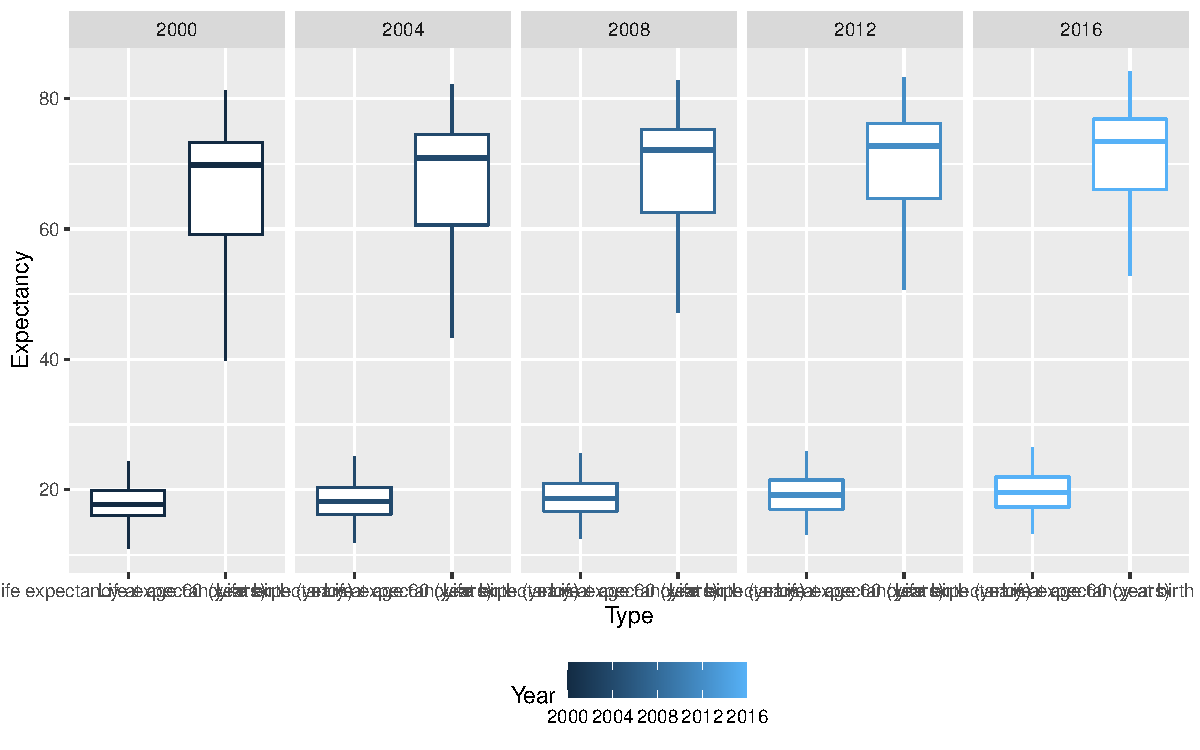
\includegraphics{ETC5513-assignment4_files/figure-latex/3box-1.pdf}
\caption{\label{fig:3box}Life expectancy at birth (years) and at age 60 (years) boxplot in 2000, 2004,2008, 2012, 2016}
\end{figure}

Table @ref(tab:3avg\_yeari) lists the average life expectancy at birth and at 60, taking into account of all countries where their life expectancy informations are available. Yearly increments at birth and at 60 represent the increasing proportion of the average each year comparing with the average of the former year. Similar to the results of boxplots, the averages had continued increasing since 2001. However, the extent of the rising pattern for average life expectancy at 60 is relatively insignificant to that at birth.

\textbackslash{}begin\{table\}

\textbackslash{}caption\{(\#tab:3avg\_yeari)Average life expectancy at birth, at age 60 (years) and their yearly increment\}
\centering

\begin{tabular}[t]{r|r|r|r|r}
\hline
Year & average LE at birth & average LE at 60 & Yearly increment at birth & Yearly increment at 60\\
\hline
2000 & 66.48956 & 18.03352 & NA & NA\\
\hline
2001 & 66.86538 & 18.17857 & 0.3758242 & 0.1450549\\
\hline
2002 & 67.07198 & 18.22033 & 0.2065934 & 0.0417582\\
\hline
2003 & 67.28516 & 18.26648 & 0.2131868 & 0.0461538\\
\hline
2004 & 67.62088 & 18.42308 & 0.3357143 & 0.1565934\\
\hline
2005 & 67.98681 & 18.52363 & 0.3659341 & 0.1005495\\
\hline
2006 & 68.44286 & 18.71978 & 0.4560440 & 0.1961538\\
\hline
2007 & 68.86374 & 18.85440 & 0.4208791 & 0.1346154\\
\hline
2008 & 69.27418 & 18.97637 & 0.4104396 & 0.1219780\\
\hline
2009 & 69.72418 & 19.10714 & 0.4500000 & 0.1307692\\
\hline
2010 & 69.94505 & 19.12143 & 0.2208791 & 0.0142857\\
\hline
2011 & 70.48626 & 19.33242 & 0.5412088 & 0.2109890\\
\hline
2012 & 70.74560 & 19.39890 & 0.2593407 & 0.0664835\\
\hline
2013 & 71.04890 & 19.51978 & 0.3032967 & 0.1208791\\
\hline
2014 & 71.24945 & 19.60110 & 0.2005495 & 0.0813187\\
\hline
2015 & 71.49725 & 19.64011 & 0.2478022 & 0.0390110\\
\hline
2016 & 71.78798 & 19.75519 & 0.2907254 & 0.1150814\\
\hline
\end{tabular}

\textbackslash{}end\{table\}
Figure @ref(fig:3avg\_yeari\_gr) exhibits the yearly improvements in average life expectancy both at birth and at 60 from 2000 to 2016. The increment for life expectancy at 60 was lower than that at birth for all times from 2000 to 2016. Nevertheless, the patterns for both of them are similar. For example, their increments in 2016 nearly drop to zero. On the next year, they both increase to the maximum increment from 2000 to 2016, as shown as the peaks.
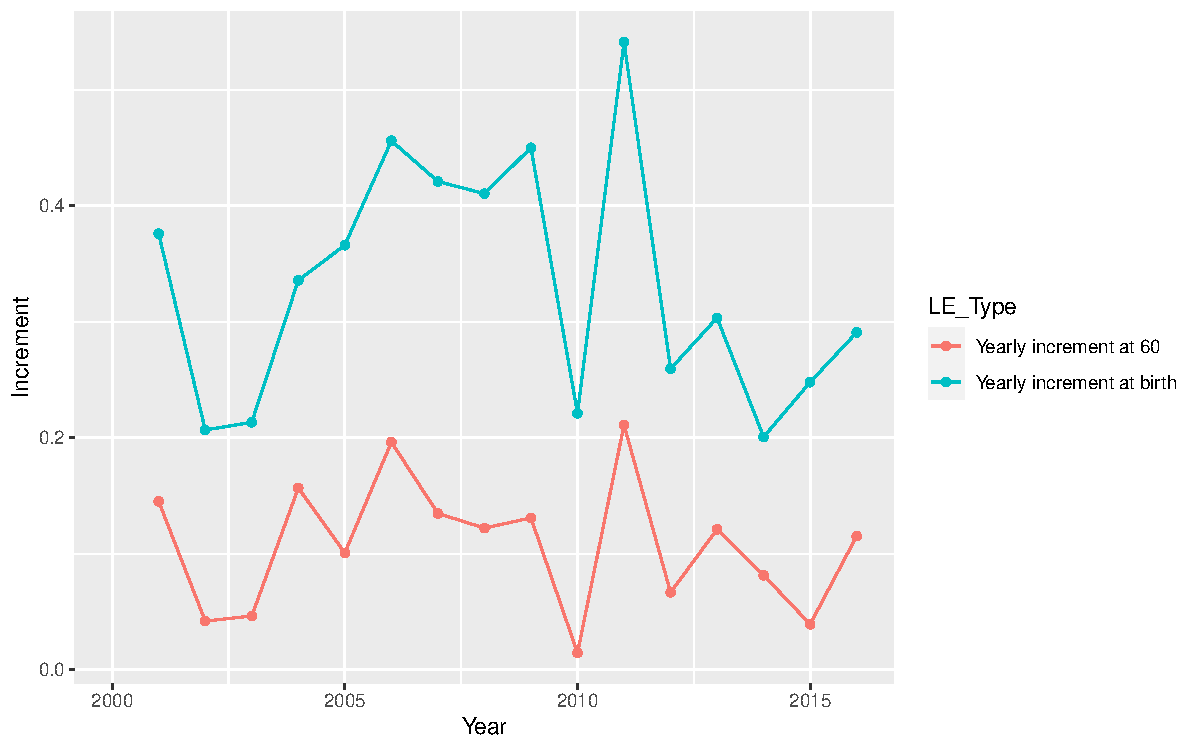
\includegraphics{ETC5513-assignment4_files/figure-latex/3avg_yeari_gr-1.pdf}

Table @ref(tab:3count\_birth\_60) contains the number of countries which had and had not met the average life expectancy from 2000 to 2016.

\textbackslash{}begin\{table\}

\textbackslash{}caption\{(\#tab:3count\_birth\_60)Number of countries met and unmet average life expectancy at birth, at age 60 (years) each year\}
\centering

\begin{tabular}[t]{r|l|r|r}
\hline
Year & meet\_avg & number\_countries\_birth & number\_countries\_60\\
\hline
2000 & met & 90 & 67\\
\hline
2000 & unmet & 92 & 115\\
\hline
2001 & met & 93 & 72\\
\hline
2001 & unmet & 89 & 110\\
\hline
2002 & met & 95 & 70\\
\hline
2002 & unmet & 87 & 112\\
\hline
2003 & met & 97 & 73\\
\hline
2003 & unmet & 85 & 109\\
\hline
2004 & met & 97 & 75\\
\hline
2004 & unmet & 85 & 107\\
\hline
2005 & met & 98 & 76\\
\hline
2005 & unmet & 84 & 106\\
\hline
2006 & met & 100 & 78\\
\hline
2006 & unmet & 82 & 104\\
\hline
2007 & met & 105 & 83\\
\hline
2007 & unmet & 77 & 99\\
\hline
2008 & met & 107 & 88\\
\hline
2008 & unmet & 75 & 94\\
\hline
2009 & met & 110 & 87\\
\hline
2009 & unmet & 72 & 95\\
\hline
2010 & met & 110 & 89\\
\hline
2010 & unmet & 72 & 93\\
\hline
2011 & met & 112 & 91\\
\hline
2011 & unmet & 70 & 91\\
\hline
2012 & met & 115 & 90\\
\hline
2012 & unmet & 67 & 92\\
\hline
2013 & met & 116 & 92\\
\hline
2013 & unmet & 66 & 90\\
\hline
2014 & met & 114 & 95\\
\hline
2014 & unmet & 68 & 87\\
\hline
2015 & met & 116 & 96\\
\hline
2015 & unmet & 66 & 86\\
\hline
2016 & met & 121 & 97\\
\hline
2016 & unmet & 62 & 86\\
\hline
\end{tabular}

\textbackslash{}end\{table\}

Figure @ref(fig:3combine\_count) combines the number of countries that had met the average life expectancy at birth, at 60 and number of countries that had not met the averages from 2000 to 2016. As years pass on, more countries had been meeting and exceeding the average life expectancy at birth and at 60 each year. However, a pheonomenon is revealed here - Although the number of countries meeting average life expectancy at 60 is lower than that at birth, the number of countries which did not meet the average is much higher. Further, since 2001, the number of countries meeting average life expectancy at birth had already surpassed that of not meeting. Yet for life expectancy at 60, it was until 2013, the number of countries meeting the average life expectancy at 60 began to exceed that of unmet number of countries.

\begin{verbatim}
## 
## Attaching package: 'gridExtra'
\end{verbatim}

\begin{verbatim}
## The following object is masked from 'package:dplyr':
## 
##     combine
\end{verbatim}

\begin{figure}
\centering
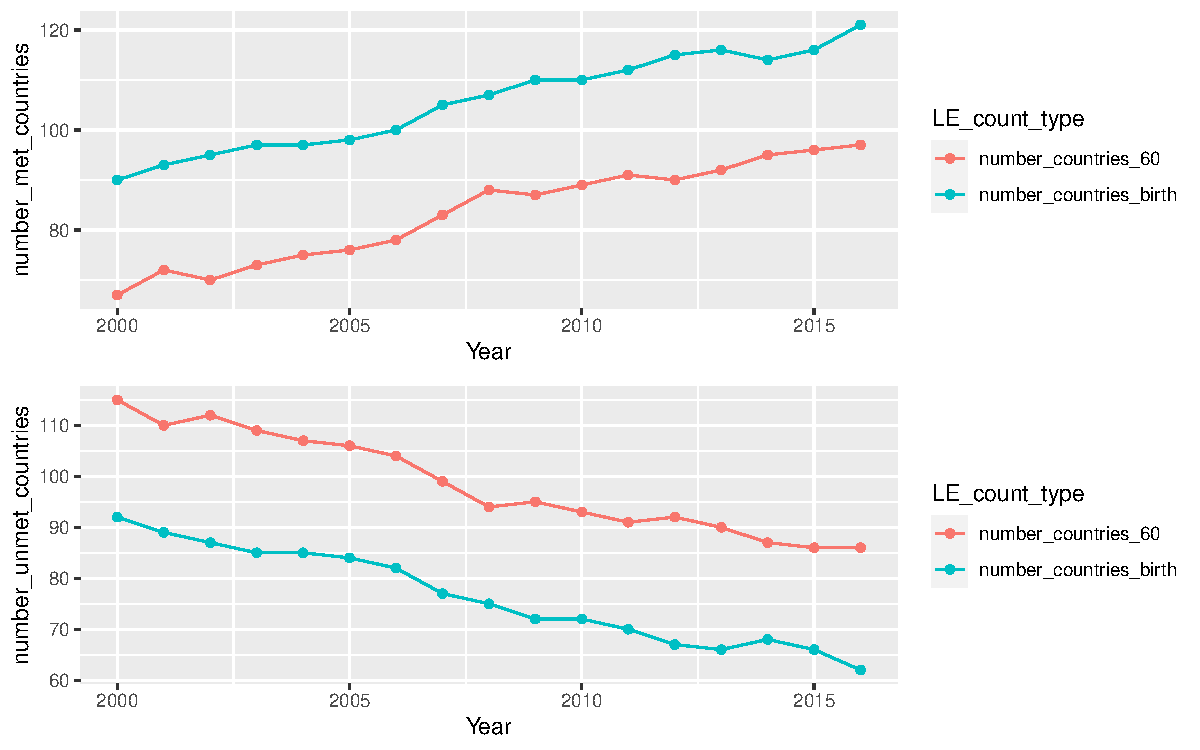
\includegraphics{ETC5513-assignment4_files/figure-latex/3combine_count-1.pdf}
\caption{(\#fig:3combine\_count)Trend of number of countries meeting and not meeting each year average LE at birth and 60}
\end{figure}

\section*{Life expectancy and Gross Domestic Product}

\printbibliography

\end{document}

